\documentclass{beamer}

\mode<presentation> {
\usetheme{AnnArbor}
}

\usepackage{graphicx}
\graphicspath{{./figures/}}
\usepackage{caption}
\usepackage{subcaption}
\usepackage{hyperref}
\hypersetup{colorlinks=true}
\usepackage{amsmath}
\usepackage{amsthm}
\usepackage{multirow}
\usepackage{siunitx}
\usepackage{biblatex}
\addbibresource{bibliography.bib}

\AtEveryBibitem{
    \clearfield{doi}
    \clearfield{isbn}
    \clearfield{issn}
    \clearlist{language}
    \clearfield{note}
    \clearfield{url}
    \clearfield{urlyear}
}

\setbeamertemplate{caption}[numbered]

\newtheorem{assumption}{Assumption}[section]
\newtheorem{proposition}{Proposition}
\newtheorem{remark}{Remark}[section]
\def\C{\mathbb C}
\def\E{\mathbb E}
\def\I{\mathbb I}
\def\P{\mathbb P}
\def\R{\mathbb R}
\def\RV{\text{RV}}
\def\Z{{\mathbb Z}}
\def\FPR{\text{FPR}}
\def\TPR{\text{TPR}}
\def\sign{{\rm sign}}
\def\ind{\perp\!\!\!\perp}
\def\seqSet{\mathcal{C}_{\alpha}}
\def\series{\xi}
\newcommand{\multiplier}[2]{\kappa_{#1}(#2)}
\newcommand{\mmultiplier}[4]{\kappa_{#1, #2}(#3, #4)}
\newcommand{\normConst}[3]{\eta_{#1}({#2}, {#3})}
\newcommand{\pred}[1]{\hat{Y}_{t + h}^{\text{(#1)}}}
\newcommand{\AROptPred}[3]{\hat{Y}_{#1 + #2}(#3)}
\newcommand{\approxAROptPred}[3]{\hat{Y}_{#1 + #2}(\hat{#3})}
\DeclareMathOperator*{\argmin}{arg\,min}
\DeclareMathOperator*{\argmax}{arg\,max}

\title[Optimal Prediction of Extreme Events]{Optimal Prediction of Extreme Events \\ with Applications to Solar Flare Forecasting}

\author{Victor Verma, Yang Chen, Stilian Stoev}
\institute[]
{
Department of Statistics \\
University of Michigan
}
\date[7/18/24]{7/18/24}

\begin{document}

\begin{frame}
    \titlepage
\end{frame}

\begin{frame}{Outline}
   \tableofcontents
\end{frame}

\section{Introduction}

\begin{frame}{Solar Flares}
    \begin{itemize}
        \item Solar flares: sudden, massive eruptions of electromagnetic radiation from the Sun's atmosphere
        \item Adverse effects of solar flares: 
        \begin{itemize}
            \item Radio blackouts
            \item Coronal mass ejection (CME) $\rightarrow$ electromagnetic pulse $\rightarrow$ electrical blackouts
            \item Solar energetic particle event (SEP) $\rightarrow$ irradiation of astronauts
        \end{itemize}
        \item Some notable incidents:
        \begin{itemize}
            \item 1989: Quebec's electrical grid was shut down for several hours
            \item 2022: Dozens of Starlink satellites were destroyed
        \end{itemize}
    \end{itemize}
\end{frame}

\begin{frame}{The X-Ray Flux}
    \begin{figure}
        \centering
        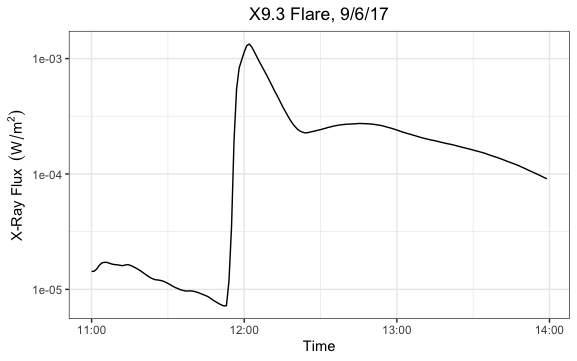
\includegraphics[scale=0.5]{flare_flux_example.png}
        \caption{The X-ray flux around the time of a strong flare.}
        \label{fig:flare_flux_example}
    \end{figure}
\end{frame}

\begin{frame}{The X-Ray Flux}
    \begin{figure}
        \centering
        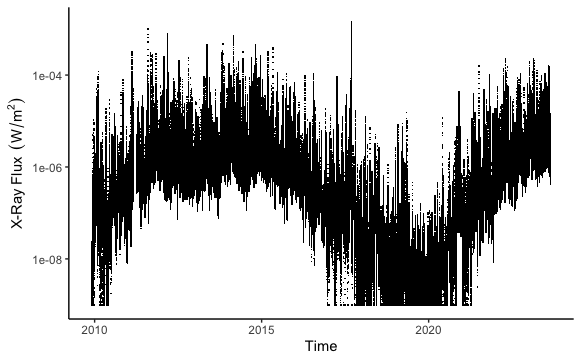
\includegraphics[scale=0.5]{flux_plot.png}
        \caption{The X-ray flux time series.}
        \label{fig:flux_plot}
    \end{figure}
\end{frame}

\begin{frame}{Flare Strength}
    Flare strength is determined by the peak (soft) X-ray flux.
    \begin{table}
        \centering
        \begin{tabular}{|c|c|}
            \hline
            Flare Class & X-Ray Flux Threshold ($\text{W} / \text{m}^2$) \\
            \hline
            A & $10^{-8}$ \\
            B & $10^{-7}$ \\
            C & $10^{-6}$ \\
            M & $10^{-5}$ \\
            X & $10^{-4}$ \\
            \hline
        \end{tabular}
        \caption{X-ray flux thresholds for the different flare classes}
        \label{tab:flare_classes}
    \end{table}

    \textbf{
        Goal:
        \begin{center}
            Forecast flares by predicting whether the flux will exceed a threshold
        \end{center}
    }
\end{frame}

\begin{frame}{Existing Work}
    Example: Deep Flare Net \cite{nishizuka2018deep, nishizuka2021oper}
    \begin{itemize}
        \item Predicts whether strong flare will occur in next 24 hours
        \item For M+ class flares, non-operational TSS = 0.8, operational = 0.24
    \end{itemize}    
    The flare forecasting problem has not been solved:
    \begin{itemize}
        \item Forecasting methods were compared in operational setting in \cite{leka2019acomII, leka2019acomIII}
        \item Goal: predict if C+ class or M+ class flare will occur in next 24 hours
        \item For both, no method attained a TSS over 0.5.
        \item ML-based methods tended to perform worse
    \end{itemize}
\end{frame}

\section{Foundations of Optimal Extreme Event Prediction}

\begin{frame}{The Statistical Problem}
    Let $Y$ be a random variable with CDF $F_Y$ and quantile function $F_Y^{-1}$. Let $X$ be a random vector in $\R^d$.

    \medskip
    
    \textbf{
    The flare forecasting problem is an instance of this general problem:
    \begin{center}
        Predict whether $Y > F_Y^{-1}(p)$ using $g(X)$ for some suitable $g$.
    \end{center}
    }
    Example:
    \begin{itemize}
        \item $Y$: flux at time $t + h$
        \item $X$: vector of fluxes at times $t, \ldots, t - \ell$
    \end{itemize}

    \medskip
    
    Assume that $F_Y$ is continuous at $F_Y^{-1}(p)$. Then $\P(Y > F_Y^{-1}(p)) = 1 - p$.
\end{frame}

\begin{frame}{Calibration of Predictors}
    Given $g$, we predict that $Y > F_Y^{-1}(p)$ when $g(X)$ lies in some set $S$.

    Indicators can be used to represent both the predictand and a predictor:
    \[
    \I(Y > F_Y^{-1}(p)), \ \I(g(X) \in S)
    \]

    Predictors should be calibrated:
    \begin{definition}
        $\I(g(X) \in S)$ is calibrated if $\P(g(X) \in S) = 1 - p = \P(Y > F_Y^{-1}(p))$.
    \end{definition}
    If $F_{g(X)}$ is continuous at $F_{g(X)}^{-1}(p)$, then $(F_{g(X)}^{-1}(p), \infty)$ is an obvious choice for $S$, as
    \[
    \I(g(X) \in S) = \I(g(X) > F_{g(X)}^{-1}(p)) = 1 - p.
    \]
\end{frame}

\begin{frame}{Optimality of Predictors}
    \begin{definition}
        $\I(g(X) \in S)$ is an optimal predictor of $\I(Y > F_Y^{-1}(p))$ if
        \begin{itemize}
            \item it is calibrated
            \item for any other calibrated predictor $\I(k(X) \in T)$,
            \begin{equation}\label{eq:optimality_cond}
                \P(Y > F_Y^{-1}(p) \mid g(X) \in S) \ge \P(Y > F_Y^{-1}(p) \mid k(X) \in T)
            \end{equation}
        \end{itemize}
    \end{definition}
    We call probabilities like those in \eqref{eq:optimality_cond} precisions and denote them by $\lambda_p$. The optimal precision is then $\P(Y > F_Y^{-1}(p) \mid g(X) \in S)$.
\end{frame}

\begin{frame}{Optimal Predictors in the General Case}
    \begin{itemize}
        \item Let $X$ and $Y$ have a joint density $f$ with respect to the Lebesgue measure on $\R^d \times \mathbb{R}$.
        \item Let $f_0$ be the conditional density of $X$ given that $Y \le F_Y^{-1}(p)$
        \item Let $f_1$ be the conditional density of $X$ given that $Y > F_Y^{-1}(p)$
    \end{itemize}
    Then
    \[
    f_0(x) = \frac{1}{p}\int_{-\infty}^{F_Y^{-1}(p)} f(x, y)\,dy, \
    f_1(x) = \frac{1}{1 - p}\int_{F_Y^{-1}(p)}^{\infty} f(x, y)\,dy
    \]
    \begin{theorem}
        Let $r(x) = f_1(x) / f_0(x)$. Suppose that $F_{r(X)}$ is continuous at $F_{r(X)}^{-1}(p)$. Then $\I(r(X) > F_{r(X)}^{-1}(p))$ is an optimal predictor of $\I(Y > F_Y^{-1}(p))$.
    \end{theorem}
\end{frame}

\begin{frame}{Optimal Predictors in Special Cases}
    \begin{theorem}
        Let $X \in \R^d$ and $\epsilon \in \R$ be independent and let $\sigma$ be a function that is positive on the range of $X$. Suppose that 
        \begin{equation}\label{eq:add_err_mod}
            Y = \mu(X) + \sigma(X)\epsilon.
        \end{equation}
        Then an optimal predictor of $\I(Y > F_Y^{-1}(p))$ is $\I(g(X) \ge F_{g(X)}^{-1}(p))$, where
        \[
        g(X) = \frac{\mu(X) - F_Y^{-1}(p)}{\sigma(X)},
        \]
        assuming that $F_{g(X)}$ is continuous at $F_{g(X)}^{-1}(p)$.
    \end{theorem}
\end{frame}

\begin{frame}{Optimal Predictors in Special Cases}
    \begin{corollary}
        When $\sigma(X)$ in \eqref{eq:add_err_mod} is constant with respect to $X$, and $F_{\mu(X)}$ is continuous at $F_{\mu(X)}^{-1}(p)$, then an optimal predictor of $\I(Y > F_Y^{-1}(p))$ is
        \[
        \I(\mu(X) \ge F_{\mu(X)}^{-1}(p)).
        \]
    \end{corollary}

    \begin{proposition}
        Let $Y = \mu(X + \delta) + \epsilon$, where $X$, $\delta$, and $\epsilon$ are independent random
        variables. If $\mu$ is increasing, and $F_X$ is continuous at $F_X^{-1}(p)$, then an optimal predictor of $\I(Y > F_Y^{-1}(p))$ is $\I(X > F_X^{-1}(p))$.
    \end{proposition}
\end{frame}

\begin{frame}{Performance Metrics}
    Let $\I(g(X) \in S)$ be a calibrated predictor of $\I(Y > F_Y^{-1}(p))$. We call
    \[
    \P(g(X) \in S \mid Y > F_Y^{-1}(p)), \ \P(g(X) \in S \mid Y \le F_Y^{-1}(p))
    \]
    the true positive rate (TPR) and false positive rate (FPR), respectively, of the predictor.

    \medskip
    
    Let $A = \{g(X) \in S\}$ and $E = \{Y > F_Y^{-1}(p)\}$. We can express the TPR and FPR in terms of the precision $\lambda_p$:
    \[
    \TPR = \P(A \mid E) = \frac{\P(A)\P(E \mid A)}{\P(E)} = \frac{(1 - p)\lambda_p}{1 - p} = \lambda_p.
    \]
    \[
    \FPR = \P(A \mid E^c) = \frac{\P(A)\P(E^c \mid A)}{\P(E^c)} = \frac{(1 - p)(1 - \lambda_p)}{p}.
    \]
\end{frame}

\begin{frame}{Performance Metrics}
    Many metrics are used to evaluate predictor performance. Two examples are the TSS and the F1 score. Again letting $\lambda_p$ be the precision, we have
    \[
    \text{TSS} := \text{TPR} - \text{FPR} = \lambda_p - \frac{(1 - p)(1 - \lambda_p)}{p} = \frac{1}{p}\lambda_p - \frac{1 - p}{p}
    \]
    and
    \[
    \text{F1} := \frac{2\lambda_p \cdot \text{TPR}}{\lambda_p + \text{TPR}} = \frac{2\lambda_p^2}{2\lambda_p} = \lambda_p
    \]
    so maximizing the precision is equivalent to maximizing the TSS and the F1 score.
\end{frame}

\section{Optimal Prediction for MA($\infty$) Models}

\begin{frame}{The Pareto Distribution}
    For a random variable $X$ with CDF $F_X$, let $\bar{F}_X = 1 - F_X$.

    \smallskip
    
    $X$ has a Pareto distribution with scale parameter $x_m > 0$ and shape parameter $\alpha > 0$ if
    \[
    \bar{F}_X(x) = \left(\frac{x}{x_m}\right)^{-\alpha}
    \]
    for all $x \ge x_m$.

    \medskip

    The Pareto distribution is considered heavy-tailed. Also, if $X \sim \text{Pareto}(x_m, \alpha)$, then $\E(X^n) = \infty$ for all $n \ge \alpha$.
\end{frame}

\begin{frame}{The Pareto Distribution}
    \begin{figure}
        \begin{subfigure}{0.5\textwidth}
            \centering
            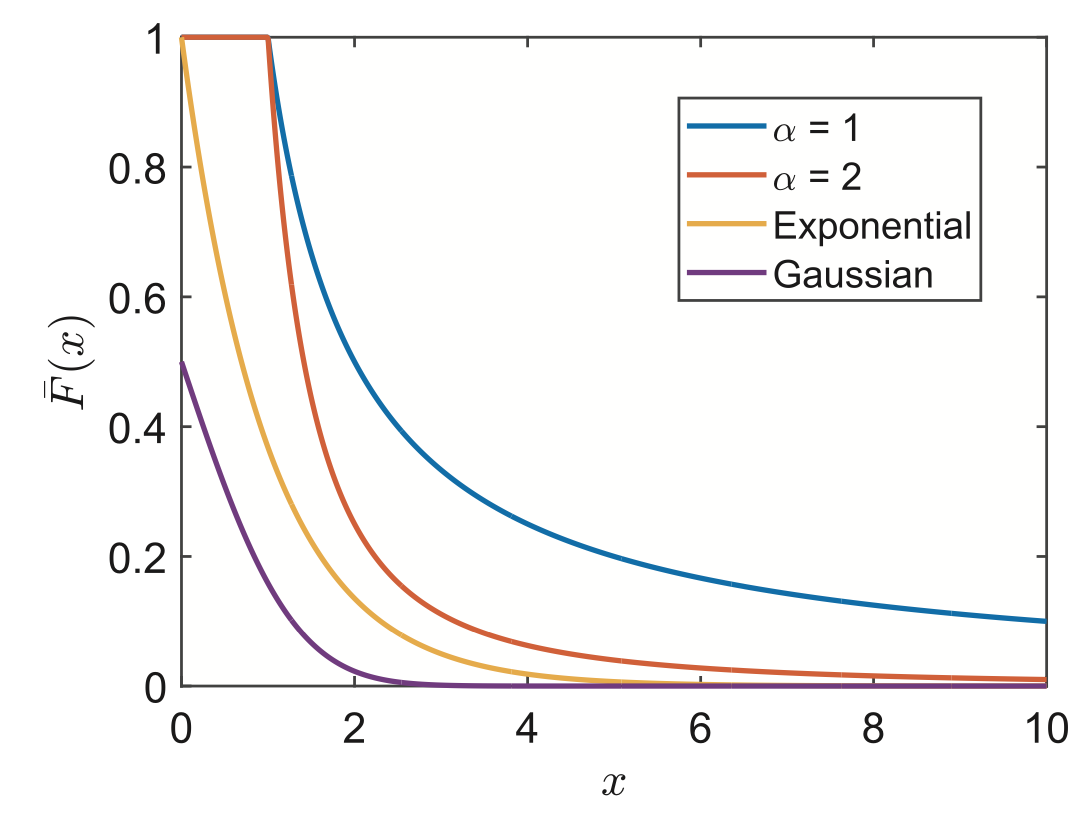
\includegraphics[width=\linewidth]{dist_tails.png}
            \caption{The axes have linear scales.}
        \end{subfigure}%
        \begin{subfigure}{0.5\textwidth}
            \centering
            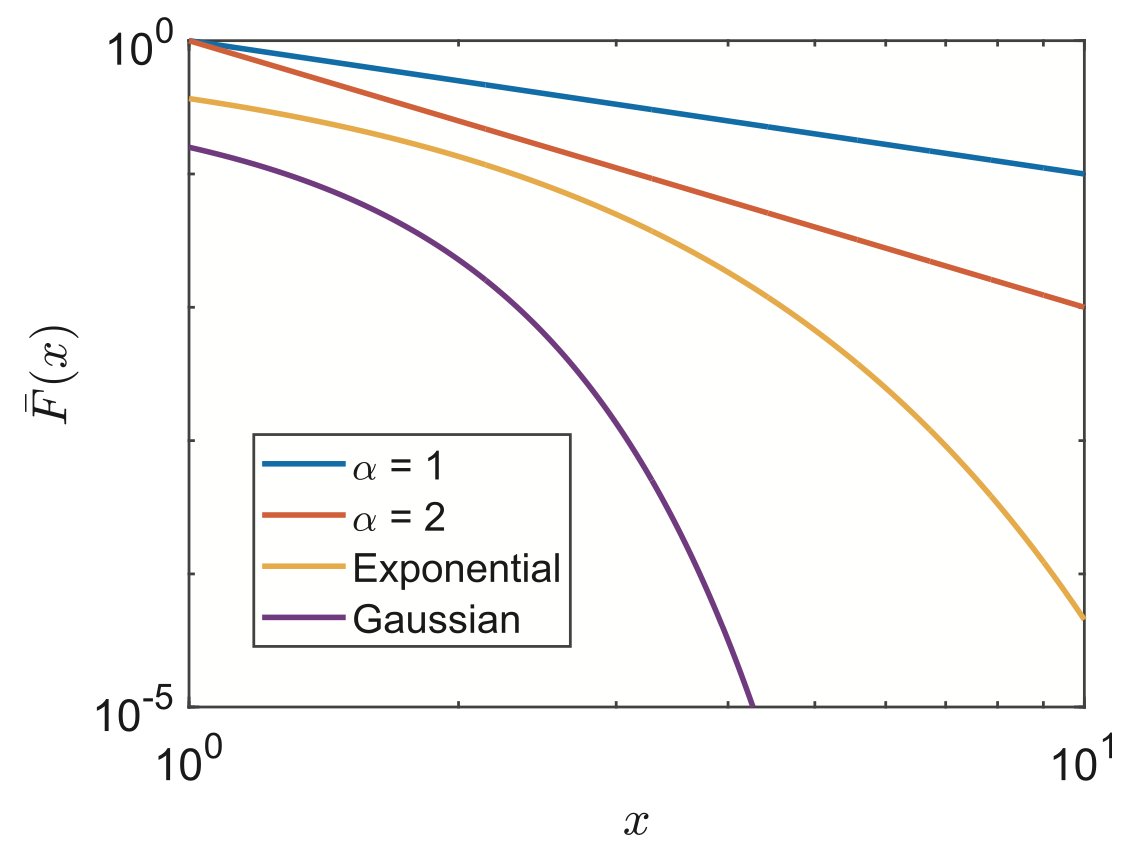
\includegraphics[width=\linewidth]{log_log_dist_tails.png}
            \caption{The axes have logarithmic scales.}
        \end{subfigure}
        \caption{A comparison of the Pareto($x_m = 1, \alpha = 1$), Pareto($x_m = 1, \alpha = 2$), Exponential(1), and Normal(0, 1) distributions (from \cite{nair2022thef}).}
    \end{figure}
\end{frame}

\begin{frame}{Regularly and Slowly Varying Functions}
    For any function $g$ defined for all large $x$, if there exists $\alpha \in \R$ such that for all large $x$,
    \[
    \lim_{t \to \infty} \frac{g(t x)}{g(t)} = x^{\alpha},
    \]
    then $g$ is called regularly varying with index $\alpha$ (written $g \in \RV_{\alpha}$). If $\alpha = 0$, then $g$ is called slowly varying.
    \begin{theorem}
        $g \in \RV_{\alpha}$ if and only if there exists $\ell \in \RV_0$ such that for all large $x$,
        \[
        g(x) = x^{\alpha}\ell(x).
        \]
    \end{theorem}
\end{frame}

\begin{frame}{Regularly Varying Random Variables}
    \begin{definition}
        Let $X$ be a random variable defined on a probability space $(\Omega, F, P)$. $X$ is regularly varying with tail index $\alpha > 0$ if
        \begin{itemize}
            \item $\bar{F}_{|X|} \in \RV_{-\alpha}$, i.e., for large $x$, $\bar{F}_{|X|}(x) = x^{-\alpha}\ell(x)$ for some $\ell \in \RV_0$.
            \item (tail balance condition) there exists $p_X \in [0, 1]$ such that
            \[
            \lim_{x \to \infty} \frac{\bar{F}_X(x)}{\bar{F}_{|X|}(x)} = p_X.
            \]
            $p_X$ is called the extremal skewness of (the distribution of) $X$.
        \end{itemize}
    \end{definition}
    Fact: $p_X > 0$ implies that $\bar{F}_X \in \RV_{-\alpha}$.
\end{frame}

\begin{frame}{The MA($\infty$) Model}
    Consider the moving average (MA) model of order $\infty$
    \begin{equation}\label{eq:ma_infty_mod}
        Y_t = \sum_{j = 0}^{\infty} a_j\epsilon_{t - j}.
    \end{equation}
    Assume that
    \begin{itemize}
        \item The $\epsilon_t$'s are iid and regularly varying with tail index $\alpha > 0$ and extremal skewness coefficient $p_{\epsilon}$.
        \begin{itemize}
            \item If $\alpha > 1$, also assume that $\E(\epsilon_t) = 0$.
        \end{itemize}
        \item $\sum_{j = 0}^{\infty} |a_j|^{\delta} < \infty$ for some $\delta \in (0, \alpha) \cap (0, 2]$.
    \end{itemize}
    Then the series in \eqref{eq:ma_infty_mod} converges absolutely almost surely.

    \textbf{
        \begin{center}
            Goal: Predict whether $Y_{t + h} > F_Y^{-1}(p)$ using $Y_s$ for $s \le t$
        \end{center}
    }
\end{frame}

\begin{frame}{The Asymptotic Precision}
    Recall that if $\I(g(X) > F_{g(X)}^{-1}(p))$ is a predictor of $\I(Y > F_Y^{-1}(p))$, then its precision is
    \[
    \lambda_p := \P(Y > F_Y^{-1}(p) \mid g(X) > F_{g(X)}^{-1}(p)).
    \]
    The asymptotic precision for $Y$ and $g(X)$ is
    \[
    \lambda = \lambda(Y, g(X)) := \lim_{p \uparrow 1} \P(Y > F_Y^{-1}(p) \mid g(X) > F_{g(X)}^{-1}(p)).
    \]
    In extreme value theory, $\lambda$ is called the tail dependence coefficient. The precision $\lambda_p$ may be hard to compute, but $\lambda$ may still be calculable with ideas from extreme value theory.
\end{frame}

\begin{frame}{Computing Asymptotic Precisions}
    Consider the class of all real sequences with the same property as $\{a_j\}$:
    \[
    \seqSet:=\Big\{ \{v_j\}\, :\, \sum_{j = 0}^{\infty} |v_j|^{\delta} < \infty \ 
    \mbox{ for some }\delta\in(0,\alpha)\cap (0,2] \Big\}.
    \]
    Introduce the following notation:
    \begin{align*}
        \multiplier{\pm}{v_j} &:= p_\epsilon\I(\pm v_j>0) + (1-p_\epsilon)\I(\pm v_j<0) \\
        \mmultiplier{\pm}{\pm}{v_j}{w_j} &:= p_\epsilon\I(\pm v_j>0, \pm w_j>0) + (1-p_\epsilon)\I(\pm v_j<0, \pm w_j<0) \\
        \normConst{\pm}{v}{h} &:= \sum_{j = h}^{\infty} \multiplier{\pm}{v_j}|v_j|^\alpha. \\
        \series(v) &:= \sum_{j = 0}^{\infty} v_j \epsilon_j.
    \end{align*}
\end{frame}

\begin{frame}{Computing Asymptotic Precisions}
    \begin{lemma}
        For all $\alpha > 0$ and sequences $v \in \seqSet$, the series $\series(v)$ converges almost surely. Moreover, $\series(v)$ is regularly varying with tail index $\alpha$ and extremal skewness
        \[
        p_{\series(v)} = \frac{\normConst{+}{v}{0}}{\sum_{j = 0}^{\infty} |v_j|^{\alpha}}.
        \]
    \end{lemma}
    \begin{lemma}
        Let $v, w \in \seqSet$. Assume that $p_{\series(v)}, p_{\series(w)} > 0$. Then
        \[
        \lambda\left(\series(v), \series(w)\right)
        = \sum_{j = 0}^{\infty} \mmultiplier{+}{+}{v_j}{w_j}\left(\frac{|v_j|^{\alpha}}{\normConst{+}{v}{0}} \bigwedge \frac{|w_j|^{\alpha}}{\normConst{+}{w}{0}}\right).
        \]
    \end{lemma}
\end{frame}

\begin{frame}{The Optimal Predictor for MA($\infty$) Models}
    The process $\{Y_t\}$ defined by \eqref{eq:ma_infty_mod} is invertible if there exists a real sequence $\{b_j\}_{j = 0}^{\infty}$ such that for all $t$, almost surely,
    \[
    \epsilon_t = \sum_{j = 0}^{\infty} b_j Y_{t - j}.
    \]

    \begin{theorem}
        Suppose $\{Y_t\}$ defined by \eqref{eq:ma_infty_mod} is invertible. Then for every $h \ge 1$, the optimal predictor of $Y_{t + h}$ based on $Y_s$, $s \le t$, is
        \[
        \pred{opt} = \sum_{j = 0}^{\infty} a_{j + h}\epsilon_{t - j}
        \]
        and $\lambda(Y_{t + h}, \pred{opt}) = \normConst{+}{a}{h} / \normConst{+}{a}{0}$, if $p_{\series(a)} > 0$.
    \end{theorem}
\end{frame}

\begin{frame}{Approximating the Optimal Predictor}
    $\pred{opt}$ is implicitly based on all past observations at time $t$ since $\epsilon_{t - j}$ is a function of $Y_s$ for all $s \le t - j$. In practice, only finitely many past observations $Y_s$, $t - \ell + 1 \le s \le t$, would be available.

    \medskip
    
    Because of invertibility, for any $u \in \Z$,
    \[
    \epsilon_u = \sum_{k = 0}^{\infty} b_k Y_{u - k}.
    \]
    Using the available observations, we approximate this by
    \[
    \tilde{\epsilon}_u = \sum_{k = 0}^{\infty} b_k Y_{u - k}\I(t - \ell + 1 \le u - k \le t).
    \]
\end{frame}

\begin{frame}{The Truncated Predictor}
    The optimal predictor based on the full history can be approximated by the ``truncated'' predictor
    \[
    \pred{trunc} = \sum_{j = 0}^{\infty} a_{j + h}\tilde{\epsilon}_{t - j}.
    \]
    This predictor can be written as a linear combination of $Y_t, \ldots, Y_{t - \ell + 1}$:
    \[
    \pred{trunc} = \sum_{j = 0}^{\ell - 1} c_j Y_{t - j},
    \]
    where $c_j, 0 \le j \le \ell - 1$, is defined by $c_j = \sum_{k = 0}^j a_{j + h - k}b_k$.
\end{frame}

\begin{frame}{The Truncated Predictor}
    Define a sequence $d = \{d_j\}_{j = 0}^{\infty}$ by
    \[
    d_j =
    \begin{cases}
        \sum_{k = 0}^j a_k c_{j - k} & \text{if $0 \le j \le \ell - 1$} \\
        \sum_{k = j - \ell + 1}^j a_k c_{j - k} & \text{if $j \ge \ell$}
    \end{cases}
    \]
    Facts about $d$:
    \begin{itemize}
        \item For $0 \le j \le \ell - 1$, $d_j = a_{j + h}$.
        \item $d \in \seqSet$.
    \end{itemize}
\end{frame}

\begin{frame}{The Truncated Predictor}
    Assume that
    \begin{itemize}
        \item For some $\gamma \in (0,1]$, $\sup_{t\in \mathbb Z} \E|\epsilon_t|^\gamma <\infty$.
        \item The sequence $a \in \seqSet$ satisfies $\sum_{k=0}^\infty |a_k| <\infty$.
    \end{itemize}
    \begin{theorem}
        (i) The truncated predictor $\pred{trunc}$ can be expressed as $\sum_{j = 0}^{\infty} d_j\epsilon_{t - j}$.
    
        (ii) If $p_{\series(a)}, p_{\series(d)} > 0$, then
        \[
         \lambda(Y_{t + h}, \pred{trunc}) = \sum_{j = 0}^{\infty} \mmultiplier{+}{+}{a_{j + h}}{d_j}\left(\frac{|a_{j + h}|^{\alpha}}{\normConst{+}{a}{0}} \bigwedge \frac{|d_j|^{\alpha}}{\normConst{+}{d}{0}}\right).
        \]
    
        (iii) If $p_{\series(a)}, p_{\series(d)} > 0$, then $\lim_{\ell \to \infty} \lambda(Y_{t + h}, \pred{trunc}) = \lambda(Y_{t + h}, \pred{opt})$.
    \end{theorem}
\end{frame}

\section{Optimal Prediction for AR($d$) Models}

\begin{frame}{The AR($d$) Model}
    Consider the autoregressive (AR) model of order $d$
    \begin{equation}\label{eq:AR_d_mod}
        Y_t = \sum_{j = 1}^d \phi_j Y_{t - j} + \epsilon_t, \ t \in \Z.
    \end{equation}
    Assume that
    \begin{itemize}
        \item the $\epsilon_t$'s are iid
        \item for all $t$, $\epsilon_t$ is independent of $Y_{t - 1}, Y_{t - 2}, \ldots$
    \end{itemize}

    \medskip

    \textbf{
        \begin{center}
            Goal: Predict whether $Y_{t + h} > F_Y^{-1}(p)$ using $Y_s$ for $s \le t$
        \end{center}
    }
\end{frame}

\begin{frame}{Stationarity of the AR($d$) Model}
    Define $\pi : \C \to \C$ by
    \[
    \pi(z) = 1 - \sum_{j = 1}^d \phi_j z^j
    \]
    If $\pi$'s roots lie outside the closed unit disk, then the AR($d$) model \eqref{eq:AR_d_mod} has a unique stationary solution that is causal:
    % Under certain conditions, this series may converge absoluteley almost surely. What conditions are those?
    \begin{equation}\label{eq:AR_d_mod_solution}
        Y_t = \sum_{j = 0}^\infty a_j \epsilon_{t - j},
    \end{equation}
    where the $a_j$'s are given by
    \[
    \sum_{j = 0}^\infty a_j z^j = 1 / \pi(z)
    \]
    when $|z| \le 1$.
\end{frame}

\begin{frame}{Two Useful Sequences}
    Let $\{Y_t\}$ be an AR($d$) stochastic process satisfying \eqref{eq:AR_d_mod}.

    \smallskip
    
    Define $\{\phi(h)\}_{h = -(d - 1)}^{\infty} \subset \R^d$ and $\{\psi(h)\}_{h = -(d - 1)}^{\infty} \subset \R^h$ as follows.
    
    When $-(d - 1) \le h \le 0$, set
    \[
    \phi_j(h) = \delta_{|h|, j}, \quad 0 \le j \le d - 1 \label{eq:phi_recur_rel1}, \quad \text{and} \quad
    \psi_j(h) = 0, \quad 1 \le j \le h
    \]
    $\delta$ being the Kronecker delta. For $h \ge 1$, define $\phi(h)$ and $\psi(h)$ by
    \begin{align*}
        \phi_j(h) &= \sum_{i = 1}^d \phi_i\phi_j(h - i), \quad 0 \le j \le d - 1 \\
        \psi_j(h) &=
        \begin{cases}
            \sum_{i = 1}^{(h - j) \wedge d} \phi_i\psi_j(h - i), & 1 \le j \le h - 1 \\
            1, & j = h
        \end{cases}
    \end{align*}
\end{frame}

\begin{frame}{Two Useful Sequences}
    Some observations:
    \begin{itemize}
        \item Let $\{e_1, \ldots, e_d\}$ be the standard basis of $\R^d$. Then
        \[
        \phi(0) = e_1, \ldots, \phi(-(d - 1)) = e_d.
        \]
        \item For $h \ge 1$, $\phi(h) = (\begin{matrix} \phi(h - 1) & \cdots & \phi(h - d) \end{matrix})\phi$.
        \item $\phi(1) = (\begin{matrix} \phi(0) & \cdots & \phi(-(d - 1)) \end{matrix})\phi = (\begin{matrix} e_1 & \cdots & e_d \end{matrix})\phi = \phi$.
    \end{itemize}
    \begin{lemma}
        (i) For all $h \ge -(d - 1)$,
        \[
        Y_{t + h} = \sum_{j = 0}^{d - 1} \phi_j(h)Y_{t - j} + \sum_{j = 1}^h \psi_j(h)\epsilon_{t + j}.
        \]
        (ii) Let $\Phi = (\begin{matrix} \phi & e_1 & \cdots & e_{d - 1} \end{matrix}) \in \R^{d \times d}$. Then $\phi(h) = \Phi^h e_1$ for all $h \ge 1$.
    \end{lemma}
\end{frame}

\begin{frame}{The Optimal Predictor for AR($d$) Models}
    \begin{theorem}
        Let $\{Y_t\}$ be the unique stationary solution of the AR$(d)$ equation in \eqref{eq:AR_d_mod}.
        The optimal predictor of $\I(Y_{t + h} > F_Y^{-1}(p))$ via
        \[
        Y_{t:(t - d + 1)} := (Y_t, \ldots, Y_{t - d + 1})^{\top}
        \]
        is $\I(\AROptPred{t}{h}{\phi} > F_{\AROptPred{t}{h}{\phi}}^{-1}(p))$, where
        \[
        \AROptPred{t}{h}{\phi} := \phi(h)^{\top}Y_{t:(t - d + 1)} = \sum_{j = 0}^{d - 1} \phi_j(h)Y_{t - j}.
        \]
    \end{theorem}
\end{frame}

\begin{frame}{Approximating the Optimal Predictor}
    \begin{itemize}
        \item Given an estimator $\hat{\phi}$ of $\phi$, the matrix $\Phi$ can be approximated by the matrix $\hat{\Phi} = (\begin{matrix} \hat{\phi} & e_1 & \cdots & e_{d - 1} \end{matrix})$.
        \item This yields plug-in approximations:
        \[
        \hat{\phi}(h) = \hat{\Phi}^h e_1 \text{ for } \phi(h), \quad \approxAROptPred{t}{h}{\phi} = \hat{\phi}(h)Y_{t:(t - d + 1)} \text{ for } \AROptPred{t}{h}{\phi}.
        \]
        \item $\phi$ can be estimated using methods like LAD and OLS estimation from a training set consisting of $n$ pairs
        \[
        (Y_t, Y_{(t - 1):(t - d)}), \ldots, (Y_{t - n + 1}, Y_{(t - n):(t - n - d + 1)}).
        \]
        \item Under certain conditions, if $\hat{\phi}$ is a LAD or OLS estimator, $\hat{\phi} \xrightarrow{\P} \phi$. See, e.g., \cite{davis1992mest}.
    \end{itemize}
\end{frame}

\begin{frame}{Consistency of the Approximation}
    \begin{theorem}
        Let $\phi$ be the coefficient vector in the AR($d$) model \eqref{eq:AR_d_mod}, and let $\hat{\phi}(n) := \hat{\phi}$ be an estimator of $\phi$, with $n$ being the size of the training set. Suppose that $\hat{\phi} \xrightarrow{\P} \phi$ as $n \to \infty$. Then $\hat{\phi}(h) \xrightarrow{\P} \phi(h)$ and $\approxAROptPred{t}{h}{\phi} \xrightarrow{\P} \AROptPred{t}{h}{\phi}$.
    \end{theorem}
    In practice, we would use a predictor of the form
    \[
    I(\approxAROptPred{t}{h}{\phi} > \hat{q}_n),
    \]
    where $\hat{q}_n$ is an estimate of $F_{\approxAROptPred{t}{h}{\phi}}^{-1}(p)$, like the $p$th sample quantile of
    \[
    \{\approxAROptPred{t}{h}{\phi}, \ldots, \approxAROptPred{t - n + 1}{h}{\phi}\}
    \]
\end{frame}

\begin{frame}{Consistency of the Approximation}
    \begin{theorem}
        Suppose that $\hat{\phi} \xrightarrow{\P} \phi$ and $\hat{q}_n \xrightarrow{\P} q := F_{\AROptPred{t}{h}{\phi}}^{-1}(p)$.
        
        Also suppose that $F_Y^{-1}(p)$ is a continuity point of $F_Y$ and that $q$ is a continuity point of $F_{\AROptPred{t}{h}{\phi}}$.
        
        Then $\I(\approxAROptPred{t}{h}{\phi} > \hat{q}_n)$ is:
        
        (i) Asymptotically calibrated, i.e., as $n \to \infty$,
        \[
        \P(\approxAROptPred{t}{h}{\phi} > \hat{q}_n) \to 1 - p = \P(Y_{t + h} > F_Y^{-1}(p))
        \]
        
        (ii) Asymptotically optimal, i.e., as $n \to \infty$,
        \[
        \P(Y_{t+h} > F_Y^{-1}(p) \mid \approxAROptPred{t}{h}{\phi} > \hat{q}_n) \to \lambda_p(Y_{t + h}, \AROptPred{t}{h}{\phi})
        \]
    \end{theorem}
\end{frame}

\section{Optimal Prediction for State-Space Models}

\begin{frame}{The State-Space Model}
    Consider the linear state-space model
    \begin{equation}\label{eq:orig_ssm}
        \begin{split}
            X_t &= \sum_{j = 1}^q A_j X_{t - j} + \delta_t \\
            Y_t &= g \left( \sum_{j = 0}^{r - 1} \beta_j^{\top} X_{t - j} \right) + \epsilon_t,
        \end{split}
    \end{equation}
    where
    \begin{itemize}
        \item $X_t \in \R^d$ and the $\delta_t$'s are iid heavy-tailed
        \item $Y_t \in \R$, $g :\R \to \R$ is increasing, and the $\epsilon_t$'s are iid heavy-tailed with tail index $\alpha > 0$
        \item the $\delta_t$'s and the $\epsilon_t$'s are independent
    \end{itemize}
\end{frame}

\begin{frame}{The State-Space Model}
    \textbf{
        \begin{center}
            Goal: Predict whether $Y_{t + h} > F_Y^{-1}(p)$ using $X_s$ for $s \le t$
        \end{center}
    }

    \medskip
    
    We may assume that $q = r$. Also, there exist $A \in \R^{dq \times dq}$ and $\beta \in \R^{dq}$ such that a solution to
    \begin{equation}\label{eq:new_ssm}
    \tilde X_t := A \tilde X_{t-1} + \tilde \delta_t\ \ \mbox{ and }\ \ Y_t = g(\beta^{\top}\tilde X_t) + \epsilon_t,
    \end{equation}
    where
    \[
    \tilde{X}_t := (X_t^{\top} \cdots X_{t - q + 1}^{\top})^{\top} \ \ \text{and} \ \
    \tilde{\delta}_t := (\begin{matrix} \delta_t^{\top} & 0 & \cdots & 0 \end{matrix})^{\top},
    \]
    is a solution to the original model \eqref{eq:orig_ssm}, so we may assume that $q = r = 1$.
\end{frame}

\begin{frame}{The Optimal Predictor for State-Space Models}
    Relation \eqref{eq:new_ssm} implies
    \[
    Y_{t + h} = g\Big( \beta^\top A^h \tilde X_t + \delta_{t,h} \Big) + \epsilon_{t+h}
    \]
    where 
    \[
    \delta_{t,h}:= \sum_{j=1}^h \beta^\top A^{h - j}\tilde  \delta_{t+j}.
    \]
    \begin{proposition}
        Let $\{(\tilde X_t,Y_t)\}$ be a solution to the model \eqref{eq:new_ssm}. Assume that
        \begin{itemize}
            \item $\tilde{\delta}_s, \ s \ge t + 1$ and $\epsilon_s, \ s \ge t + 1$ are independent of $\tilde{X}_s, \ s \le t$
            \item $\tilde X_t$, $\delta_{t, h}$, and $\epsilon_{t+h}$ have densities
        \end{itemize}
        The optimal predictor of $\I(Y_{t+h}> F_{Y_{t+h}}^{-1}(p))$
        via $\tilde X_s, s\le t$ is $\I(\beta^\top A^h\tilde X_t > F_{\beta^\top A^h\tilde X_t}^{-1}(p))$.
    \end{proposition}
\end{frame}

\begin{frame}{A Simulation Study}
    Data was generated from the state-space model
    \begin{align*}
        X_t &= \sum_{j = 1}^5 0.5^j I_{16}X_{t - j} + \delta_t \\
        Y_t &= \sum_{j = 0}^4 0.5^j 1_{16}^{\top}X_{t - j} + \epsilon_t
    \end{align*}
    where
    \begin{itemize}
        \item $X_t \in \R^{16}$, $\delta_t \sim t_{\nu_{\delta}}(0, I_{16})$
        \item $Y_t \in \R$, $\epsilon_t \sim t_{\nu_{\epsilon}}$
        \item the $\delta_t$'s and $\epsilon_t$'s are mutually independent
    \end{itemize}
\end{frame}

\begin{frame}{A Simulation Study}
    Let 
    \[
    A =
    \left(
    \begin{matrix}
        0.5 \cdot I_{16} & 0.5^2 I_{16} & 0.5^3 I_{16} & 0.5^4 I_{16} & 0.5^5 I_{16} \\
        I_{16} & 0 & 0 & 0 & 0 \\
        0 & I_{16} & 0 & 0 & 0 \\
        0 & 0 & I_{16} & 0 & 0 \\
        0 & 0 & 0 & I_{16} & 0
    \end{matrix}
    \right), \
    \beta =
    \left(
    \begin{matrix}
        1_{16} \\
        0.5 \cdot 1_{16} \\
        0.5^2 1_{16} \\
        0.5^3 1_{16} \\
        0.5^4 1_{16}
    \end{matrix}
    \right)
    \]
    \[
    \tilde{X}_t = 
    \left(
    \begin{matrix}
        X_t^{\top} & X_{t - 1}^{\top} & X_{t - 2}^{\top} & X_{t - 3}^{\top} & X_{t - 4}^{\top}
    \end{matrix}
    \right)^{\top}
    \]
    The optimal predictor of $\I(Y_{t + 1} > F_{Y_{t + 1}}^{-1}(p))$ is $\I(\beta^{\top} A\tilde{X}_t > F_{\beta^{\top} A\tilde{X}_t}^{-1}(p))$.
\end{frame}

\begin{frame}{A Simulation Study}
    Training and test sets were of the form
    \[
    \left(
    \begin{matrix}
    X_1^{\top} & \cdots & X_{-3}^{\top} & Y_2 \\
    \vdots & \ddots & \vdots & \vdots \\
    X_n^{\top} & \cdots & X_{n - 4}^{\top} & Y_{n + 1} \\
    \end{matrix}
    \right)
    =
    \left(
    \begin{matrix}
    \tilde{X}_1^{\top} & Y_2 \\
    \vdots & \vdots \\
    \tilde{X}_n^{\top} & Y_{n + 1} \\
    \end{matrix}
    \right).
    \]

    Given a new observation $\tilde{X}_*$, predict that $Y_*$ is extreme if $\beta^{\top} A\tilde{X}_*$ is above the $p$th sample quantile of $\{\beta^{\top} A\tilde{X}_1, \ldots, \beta^{\top} A\tilde{X}_n\}$.
\end{frame}

\begin{frame}{A Simulation Study}
    \begin{figure}[h!]
        \centering
        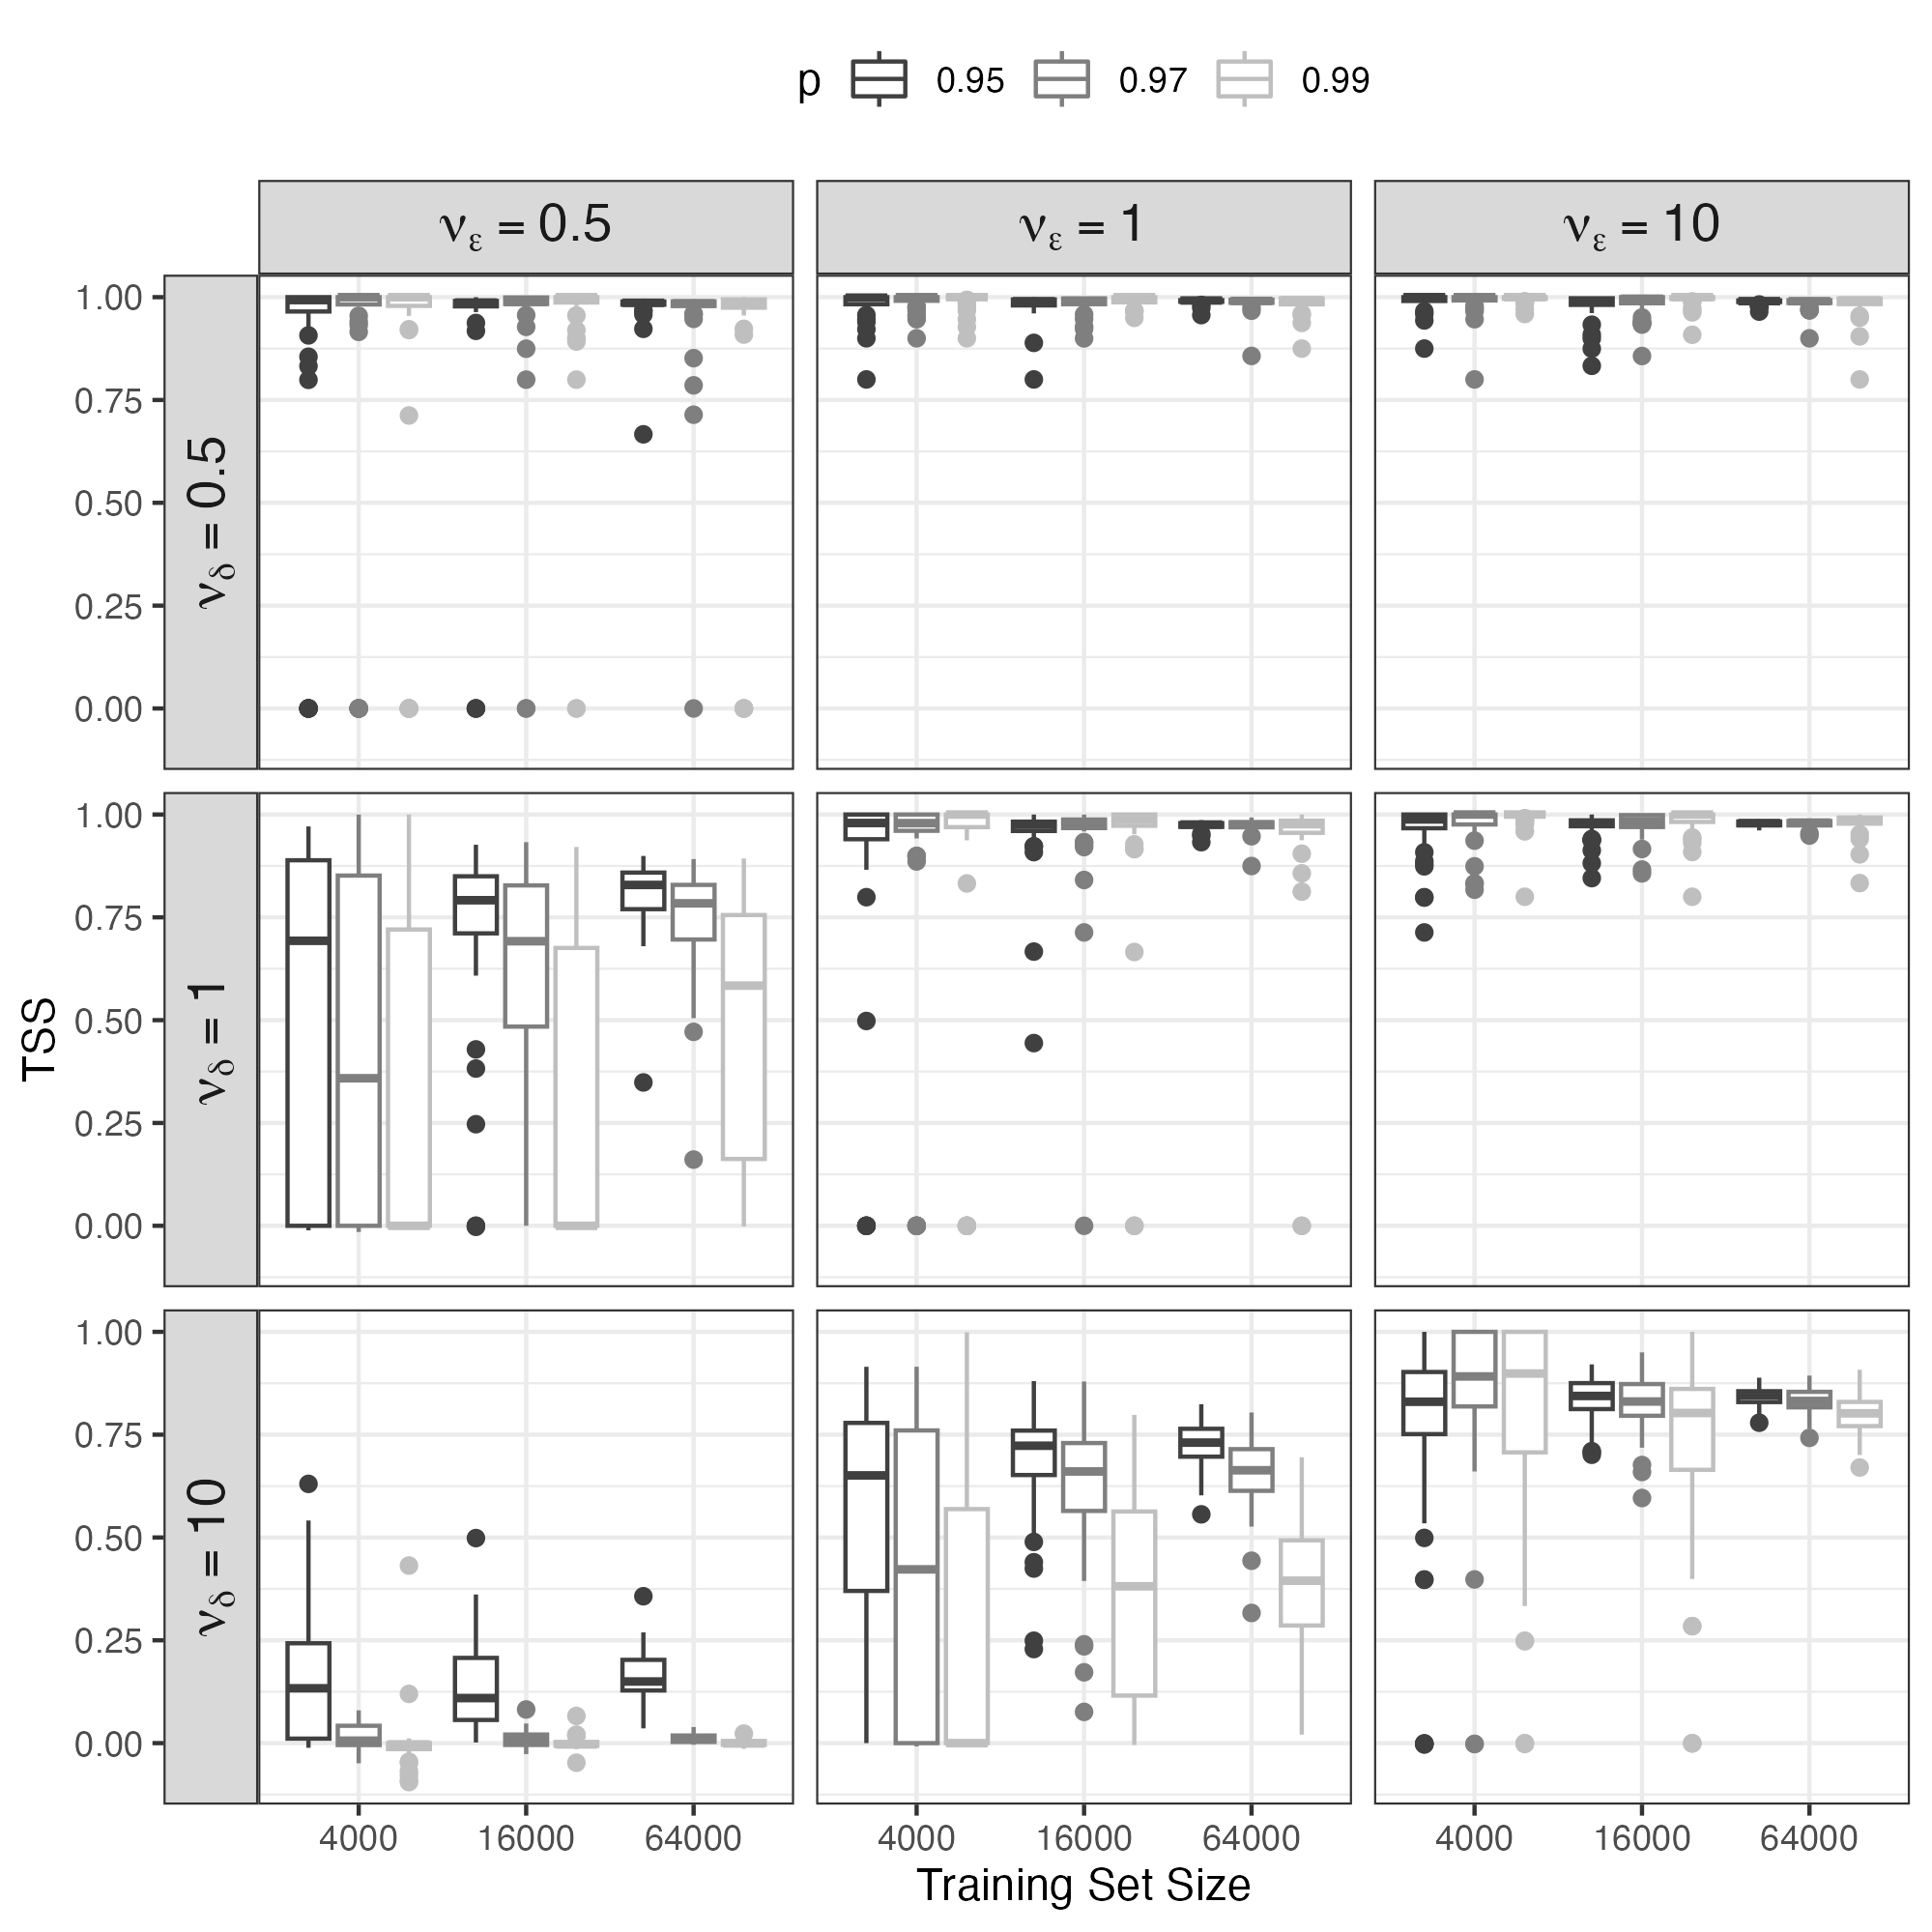
\includegraphics[scale=0.4]{sim_study07.png}
        \caption{Results of the simulation study.}
        \label{fig:sim_study07}
    \end{figure}
\end{frame}

\begin{frame}[allowframebreaks]{References}
    \printbibliography
\end{frame}

\section{Appendix}

\begin{frame}{HEK Entry, 9/6/17 X9.3 Flare}
    \begin{figure}
        \centering
        
\includegraphics[scale=0.3]{hek_entry_20170906.png}
        \caption{Heliophysics Events Knowledgebase (HEK) entry, 9/6/17 X9.3 flare.}
        \label{fig:hek_entry}
    \end{figure}
\end{frame}

\begin{frame}{Soft X-Ray Flux Values, 9/6/17 X9.3 Flare}
    \begin{figure}
        \centering
        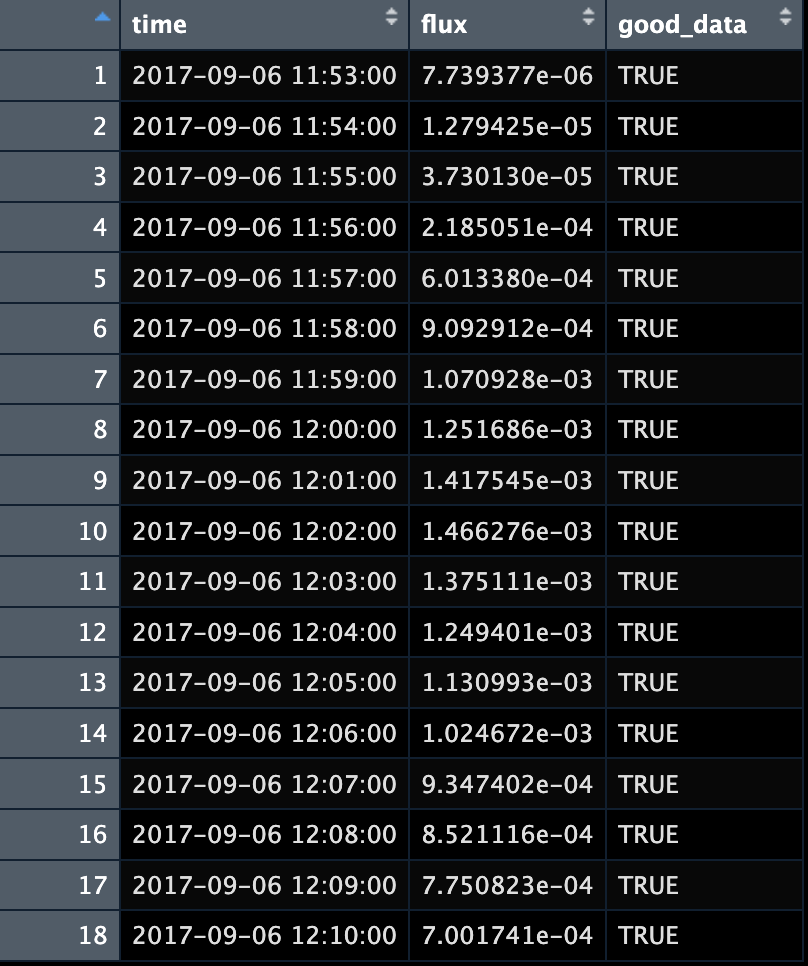
\includegraphics[scale=0.4]{flux_vals_20170906.png}
        \caption{Soft X-Ray Flux Values, 9/6/17 X9.3 Flare.}
        \label{fig:flux_vals_20170906}
    \end{figure}
\end{frame}

\end{document}